\documentclass[11pt,letterpaper]{article}
\usepackage[english]{babel}
\usepackage[utf8]{inputenc}
\usepackage{fancyhdr}
\usepackage[margin=1in]{geometry}
\usepackage{enumitem}
\usepackage{amsmath}
\usepackage{graphicx}
\usepackage{setspace} 
\onehalfspacing
 
\pagestyle{fancy}
\fancyhf{}
\lhead{STAT 423 HW 2}
\rhead{Nan Tang (1662478)}
\rfoot{Page \thepage}
 

\title{STAT 423 Homework 1}
\author{Nan Tang 1662478}
\date{\today}
 
\begin{document}
\maketitle

\section*{Problem 1}
\subsection*{a}
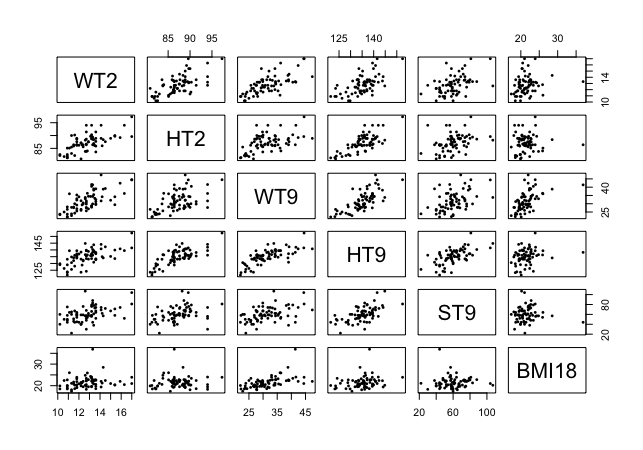
\includegraphics[scale=0.7]{1-a-1.png}
\begin{verbatim}
            WT2        HT2       WT9       HT9         ST9       BMI18
WT2   1.0000000 0.64454954 0.6925390 0.6071247 0.451581158 0.190947873
HT2   0.6445495 1.00000000 0.5229277 0.7383562 0.361724146 0.042573733
WT9   0.6925390 0.52292768 1.0000000 0.7276123 0.453004062 0.545925753
HT9   0.6071247 0.73835617 0.7276123 1.0000000 0.603368147 0.236907969
ST9   0.4515812 0.36172415 0.4530041 0.6033681 1.000000000 0.005603061
BMI18 0.1909479 0.04257373 0.5459258 0.2369080 0.005603061 1.000000000
\end{verbatim}

\noindent We can perceive from the scatter plot that the correlations between response BMI18 and predictors as ST9, HT9, HT2, WT2 are not very strong. A positive correlation might exist between BMI18 and WT9. Value of correlation coefficients reflect similar results. The coefficients between BMI18 and WT2, HT2, HT9 ST9 are less than 0.25, while some of them are close to zero. Coefficients between BMI18 and WT9 is 0.55, implying correlation may exist. \\

\noindent The patterns of scatter plot show that positive correlation may exist between WT2 and HT2, WT9, HT9. In fact, correlation coefficient between them are all greater than 0.6, providing evidence that correlation may exist. Positive correlation may also exist between HT2 and HT9, between WT9 and HT9. 

\subsection*{b}
\noindent Summary of model $E(BMI18 | WT9, ST9)$
\begin{verbatim}
Call:
lm(formula = BMI18 ~ WT9 + ST9, data = bgs_girls)

Residuals:
    Min      1Q  Median      3Q     Max 
-4.1736 -1.2146 -0.2474  1.1231 11.2834 

Coefficients:
            Estimate Std. Error t value Pr(>|t|)    
(Intercept) 14.63878    1.54661   9.465 5.66e-14 ***
WT9          0.32418    0.05151   6.293 2.72e-08 ***
ST9         -0.05552    0.01983  -2.799  0.00668 ** 
---
Signif. codes:  0 ‘***’ 0.001 ‘**’ 0.01 ‘*’ 0.05 ‘.’ 0.1 ‘ ’ 1

Residual standard error: 2.222 on 67 degrees of freedom
Multiple R-squared:  0.3715,	Adjusted R-squared:  0.3528 
F-statistic:  19.8 on 2 and 67 DF,  p-value: 1.747e-07
\end{verbatim}

\noindent Summary of model $E(BMI18 | HT2, WT2, HT9, WT9, ST9)$
\begin{verbatim}
Call:
lm(formula = BMI18 ~ ., data = bgs_girls)

Residuals:
    Min      1Q  Median      3Q     Max 
-5.0948 -1.2186 -0.2533  1.0090 10.4951 

Coefficients:
             Estimate Std. Error t value Pr(>|t|)    
(Intercept) 30.855335   8.781156   3.514 0.000817 ***
WT2         -0.317779   0.278736  -1.140 0.258505    
HT2         -0.193997   0.130819  -1.483 0.142996    
WT9          0.419762   0.075211   5.581  5.2e-07 ***
HT9          0.008057   0.096344   0.084 0.933613    
ST9         -0.044416   0.022219  -1.999 0.049853 *  
---
Signif. codes:  0 ‘***’ 0.001 ‘**’ 0.01 ‘*’ 0.05 ‘.’ 0.1 ‘ ’ 1

Residual standard error: 2.14 on 64 degrees of freedom
Multiple R-squared:  0.4431,	Adjusted R-squared:  0.3996 
F-statistic: 10.19 on 5 and 64 DF,  p-value: 3.294e-07
\end{verbatim}

\noindent At the significance level of $5 \%$, none of the estimates in model 2 but not in model 1 is significant (their p-values are all greater than 0.05). 

\subsection*{c}
\subsection*{i}
\noindent The F-statistic for testing $H_0: \beta_{HT2}, \beta_{WT2}, \beta_{HT9} = 0$ is 
\begin{align*}
F = (\frac{SSE(reduce) - SSE(full)}{df(reduce) - df(full)}) / (\frac{SSE(full)}{df(full)})
\end{align*}
\noindent Where $SSE(reduce)$ and $SSE(full)$ are error sum of squares for two models. $df(reduce) = n - 3$, $df(full) = n - 6$.

\noindent I calculated $SSE(reduce)$ and $SSE(full)$ by summing up square of residuals of two models, they are $SSE(reduce) = 330.7$, $SSE(full) = 293.04$ \\
\begin{align*}
F = \frac{(SSE(reduce) - SSE(full)) / (6 - 3)}{SSE(full) / (n - 6)} = 2.742
\end{align*}

\noindent Using R function $anova(fit1, fit2)$ could also compare these two models. The result of F-statistic in $anova$ function is 2.742 as well. 

\subsection*{ii}
\noindent The F-statistic follows an F distribution. The degree freedom of numerator is $df(reduce) - df(full) = 6-3=3$. The degree freedom of denominator is $df(full) = n - 6  = 64$ \\
\noindent Therefore, under the null hypothesis, the F-statistic follows distribution of $F_{df_1=3, df_2=64}$.

\subsection*{iii}
\noindent The p-value of this F-statistic under null hypothesis is $0.05037 $, which is slightly greater than $0.05$. Therefore, at the significance level of $0.05$, the observation fail to provide strong evidence against the null hypothesis that says $HT2, WT2, HT9$ have no significant effect on response. 

\subsection*{iv}
\noindent The result of anova test shows predictors $HT2, WT2, HT9$ are unlikely to have significant effect on the response. I will choose the reduced model which includes predictors of only $ST9$ and $WT9$, for a larger degree of freedom. 

\subsection*{d}
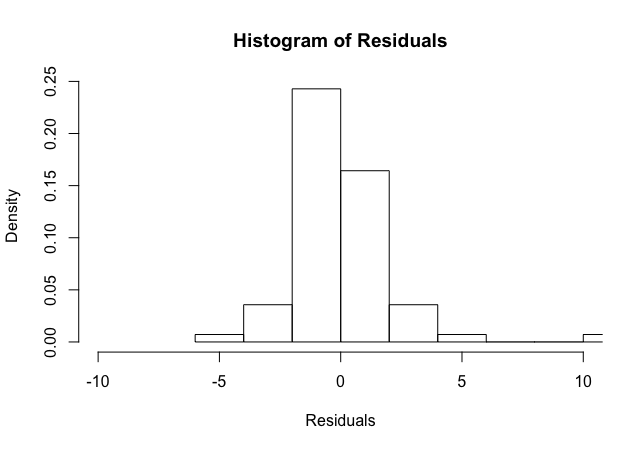
\includegraphics[scale=0.7]{1-d-1.png}

\noindent Except for one outlier, the overall distribution of residual shows a bell shape and is approximately symmetric around zero. Therefore, the normality assumption of error is not violated. 

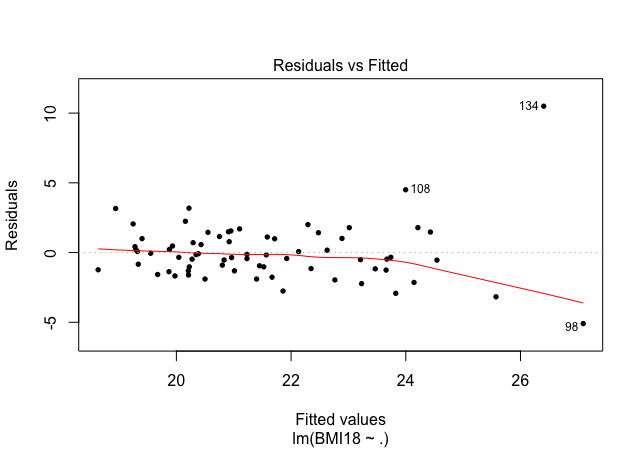
\includegraphics[scale=0.7]{1-d-2.png}
\noindent From the TA plot, we can perceive the residuals of fitted values that are lower than 24 scattered around zero line with similar width, thereby have constant variance. However, for residuals that corresponding to fitted value greater than 24, several outliers are far away from the horizontal zero line, leading the change on variance of residuals. Overall, for the appearance of these outliers on high end, the constant variance assumption is violated.

\subsection*{e}
\begin{align*}
MSE &= \frac{RSS}{df(redisual)} = \frac{\sum_i^n (y_i - \hat{y_i})^2}{n} \\
\sum_i^n (y_i - \hat{y_i})^2 &= 293.04 \\
MSE &= \frac{293.04}{70} \approx 4.186
\end{align*}
\begin{align*}
\hat{\sigma}^2 &= \frac{SSE}{df(residual)} = \frac{293.04}{70 - 6} = 4.58 \\
\hat{\sigma} &= \sqrt{4.58} = 2.14
\end{align*}
Sample $MSE$ is 4.186, while $\hat{\sigma}^2 = 2.14$. 

\subsection*{f}
\begin{enumerate}[label=\roman*.]
\item If adjust the data using bonferroni method, the null hypothesis $iv, H_0: \beta_{WT9} = 0$ will be rejected at level $0.1$. 
\item At the level of 0.1, using holm correction, only $iv, H_0: \beta_{WT9} = 0$ will be rejected. 
\item At FDR level of 0.1, using Benjamini-Hochberg procedure, only $iv, H_0: \beta_{WT9} = 0$ will be rejected.
\end{enumerate}

\section*{Problem 2}
\subsection*{a}
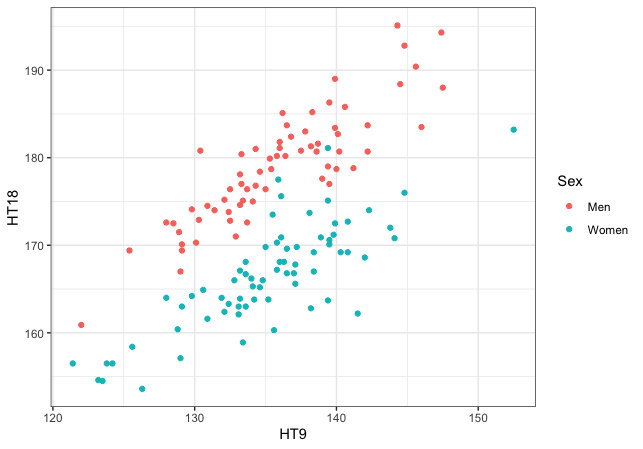
\includegraphics[scale=0.7]{2-a-1.png}

\noindent It is reasonable to include sex as a predictor. The cluster of men is distinct from the cluster of women. Given same value of $HT9$, men are clearly higher in mean of $HT18$ than women. 

\subsection*{b}
\begin{enumerate}[label=\roman*.]
\item The intercept for women in the linear regression model is 36.821 cm.
\item The predicted value for the girl who is 135 in 9 year-old is 166.429 cm.
\item The predicted average change on $HT18$, where $HT9$ from 135 to  137, is equal to the change on fitted value. The fitted value for girl whose $HT9 = 137$ is 168.349 cm. Therefore, the predicted average change is $168.349 - 166.429 = 1.92 cm$
\item Let $\beta_{sex} = E(HT18 | HT9, Sex=women) - E(HT18 | HT9, Sex=men)$. The $95 \%$ confidence interval for $\beta_{sex}$ can be represented by 
\begin{align*}
\hat{\beta_{sex}} - se \cdot t_{0.95, 136-3} &< \beta_{sex} < \hat{\beta_{sex}} + se \cdot t_{0.95, 136-3} \\
-12.67 &< \beta_{sex} < -10.72
\end{align*}
\noindent The $95 \%$ difference in HT18 between men and women is $[-12.67, -10.72]$. 
\item My suspicion in part a is right, sex is a significant categorical predictor. The p-value for $\hat{\beta_{sex}}$ under the null hypothesis is much smaller than 0.05, therefore, at the level of 0.05, I will reject the null hypothesis that $\beta_{sex} = 0$.  Base the $95 \%$ confidence interval I calculated, zero does not fall in the interval $[-12.67, -10.72]$, it is a significant evidence against the null hypothesis. 
\end{enumerate}

\subsection*{c}
\begin{enumerate}[label=\roman*.]
\item There are 3 parameters in model fit.height; 4 parameters in model fit.height2; 6 parameters in model fit.height3; 8 parameters in model fit.height4.
\item The predicted height at age 18 for girl according to fit.height2 model is 166.55; according to fit.height3 is 167.19; according to fit.height4 is 167.35. 
\item The F-statistic for comparing fit.model and fit.height2 is 0.11, with p-value of 0.74. At the significance level of 0.1, we cannot reject the null hypothesis that $H_0: \beta_{HT2} = 0$. Therefore, I will opt for the first model as preferred. 
\item The p-value for comparing fit.height4 and fit.height3 is $0.75 > 0.1$, then we continue the procedure. The p-value for comparing fit.height3 and fit.height2 is $0.054 < 0.1$. At the 0.1 level, the anova test provides significant evidence against the null hypothesis, i.e. two-way interactions have significant effects on response. Therefore, by this procedure, I will opt for fit.height3 as preferred model. 
\item The SSE's for fit.height, fit.height2, fit.height3, fit.height4 are respectively \\
$1566.896, 1565.579, 1496.882, 1490.061$.\\
Degrees of freedom are respectively $133, 132, 130, 128$. \\
Note that $\hat{\sigma} = \sqrt{\frac{SSE}{df(residual)}}$, and let $\hat{\sigma_1}$ denotes estimated variance for model 1.\\
$\hat{\sigma_1} = 3.43,  \hat{\sigma_2} = 3.44, \hat{\sigma_3} = 3.39, \hat{\sigma_4} =3.41 $ \\
The model fit.height3 has the lowest estimated variance on error, therefore, base on $\hat{\sigma}$, I prefer fit.height3 that includes only two-way interactions. 


\end{enumerate}









\end{document}